\chapter{Mathematical appendix \label{apx:maths}}

\section{Marginal analysis \label{sec:marginalapx}}

`Marginal' just means the first derivative of some quantity. Here is one example from utility and one from production. To start with the Cobb Douglas function discussed in section \ref{sec:utilityintro}: if one quantity is held constant, the other's diminishing marginal utility can be seen from graphing the partial derivative, $\frac{\partial U}{\partial f}=\frac{\sqrt{M}}{2\sqrt{F}}$ - see figure \ref{fig:dmu_cobbd}, where $M$ is set to one. The change in utility per unit diminishes (so $U''<0$); as more is consumed, each extra unit becomes less `satisfying'. Note, this makes sense given what has been said about the Cobb Douglas exhibiting basic `love of variety': if $M$ is held constant as $F$ increases, `variety' is actually dropping away from a perfect mix of the two.

\begin{figure}[h!]
\centering
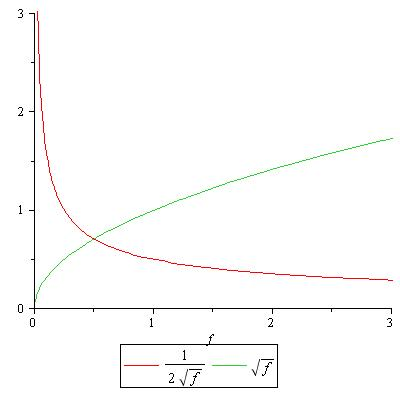
\includegraphics[width=0.5\columnwidth]{ChapterEcon/figures/DMU_cobbdouglas}%
\caption{Total and marginal utility for a $\delta=\frac{1}{2}$ Cobb Douglas utility function, holding $M$ constant at 1.}%
\label{fig:dmu_cobbd}%
\end{figure}

As discussed, the same kinds of functions are used for firms and so the same principles hold. The canonical result for firms is that output should be set where marginal cost equals marginal revenue ($MC=MR$). This is a straightforward intuition: a firm increases output by one unit. If the extra cost is lower than the extra revenue, they can still make money. If the cost is higher than the extra revenue, they would lose money. So this directs them to the point where any change in cost exactly matches the change in revenue: $MC = MR$. (For this to work, the firm's change in output cannot affect prices: see section \ref{sec:marketstructure}.)

%The meaning of `marginal' should now be clear enough. Chapter \ref{chapter:ABM} looks at the issue in more depth; for example, it is easy enough to say `a firm increases output by one unit', but how is that to happen in an agent context?
%This doesn't tell us whether TC > TR� the rule works fine for perfect competition, but otherwise�

\section{Constrained optimisation \label{sec:constrainedopt}}

\subsection{Use of constrained optima}

As section \ref{sec:constrained} outlined, constrained optimisations are used for three different utility functions: the Cobb Douglas, the Engel function and the \gls{ces} function. The first of these is commonly used in the economic literature. The \gls{ces} optimisation was derived from Brakman \emph{et al}'s constraint of a \gls{ces} function for a single good by substituting the price index back in and rearranging;see \citealt{brakman_new_2009} pp.94. The Engel function was worked out, and serves as a useful illustration of the process of using the Lagrangian multiplier to deduce equations for optimal good demand. The principle is simple enough: the constraint slices through the utility function and the partials all identify a simultaneous equation where utility is maximised. It is then just a matter of working with the simultaneous equation to find the values needed - not always possible, but doable for the Engel function. The next section runs through the process.

\subsection{Constraining the Engel function}

The Engel utility function is:

\begin{equation}
U = F^{\delta}(\gamma+M)^{1-\delta}\label{eq:engel4lag}
\end{equation}

The variables are: $U$ is utility; $F$ the necessity good; $M$ the luxury good. $\gamma$ controls the point at which demand for luxury good starts. $\delta$ is the share parameter which, as discussed in section \ref{sec:utilitynengelslaw} does not work quite perfectly in that job as it does for the Cobb Douglas, since the share is affected by $\gamma$.

The budget that will be constraining the Engel function includes the price for both goods:

\begin{equation}
Y = F \cdot p_f + M \cdot p_m\label{eq:engel4lagbudget}
\end{equation}


Equations \eqref{eq:engel4lag} and \eqref{eq:engel4lagbudget} go into the Lagrangian function. \eqref{eq:engel4lagbudget} is set to zero:

\begin{equation}
L = F^\delta(\gamma + M)^{1-\delta}+\lambda(Y-F \cdot p_f - M \cdot p_m) \label{eq:engelLagfunct}
\end{equation}

Find the partial differentials for $F$, $M$ and $\lambda$ and set to zero:

\begin{equation}
\frac{\delta L}{\delta F} = \delta F^{\delta-1} \cdot (\gamma+M)^{1-\delta}-\lambda p_f  = 0\label{eq:engelpartialF}
\end{equation}

\begin{equation}
\frac{\delta L}{\delta M} = (1-\delta) F^\delta \cdot (\gamma+M)^{-\delta}-\lambda p_m = 0\label{eq:engelpartialM}
\end{equation}

\begin{equation}
\frac{\delta L}{\delta \lambda} = Y-F\cdot p_f - M \cdot p_m = 0\label{eq:engelpartiall}
\end{equation}

\eqref{eq:engelpartialF} and \eqref{eq:engelpartialM} can be divided and simplified to give:

\begin{equation}
\frac{\delta(\gamma+M)}{F-\delta F} = \frac{p_f}{p_m}\label{eq:engeldiv}
\end{equation}

Finding a substitution to go into \eqref{eq:engelpartiall} will help produce values for $F$ and $M$. This can be achieved from \eqref{eq:engeldiv} by rearranging until it is in terms of $F \cdot p_f$:

\begin{equation}
F \cdot p_f = \frac{p_m \cdot \delta (\gamma + M)}{1-\delta} \label{eq:engeltofpf}
\end{equation}

Substituting into \eqref{eq:engelpartiall} and rearranging in terms of $M$ gives the first constrained good quantity:

\begin{equation}
M = \frac{Y\cdot(1-\delta)}{p_m} - \delta \gamma \label{eq:englagMopt}
\end{equation}

The same can be done for $F$ by rearranging \eqref{eq:engeldiv}, subsituting into \eqref{eq:engelpartiall} and rearranging again:

\begin{equation}
F = \frac{\delta (Y + p_m \cdot \gamma)}{p_f}\label{eq:englagFopt}
\end{equation}

As section \ref{sec:constrained} explained, these both become the Cobb Douglas constrained optima when $\gamma = 0$: in \eqref{eq:englagMopt} the subtracted term $\delta \gamma$ disappears; in  \eqref{eq:englagFopt}, the term $p_m \cdot \gamma$ becomes zero, taking $p_m$ with it, so the optimum for $F$ again is only dependent on the price of $F$, not the price of both.


\begin{comment}
\section{Core model overview \label{sec:coremodelapx}}

There are a number of different outlines in the literature; here, terminology and choice of parameter names come from \citeauthor{brakman_new_2009}, but to begin with, whichever approach is simplest is used. Krugman's original paper \citep{krugman_increasing_1991} is, of course, a key source - however, \citeauthor{brakman_new_2009} discuss hidden assumptions in much finer detail, and Brakman is also used by Fowler to build his agent version.
%Other versions are discussed in section \cmt{which section for discussion of other core model versions?}, as they each approach the problem from slightly different points of view. 

The usual approach to describing the \gls{coremodel} is to follow the logical path of the mathematical argument, beginning at the micro level and building up towards the model's conclusions. While this is perfectly sensible mathematically, it is not a particularly good way to open the bonnet and get a clear view of its workings. This section attacks the problem in reverse, starting with the three simultaneous equations toward the endpoint of the analytic argument. These equations are the `operational' elements - that is, they can be used to directly produce simulation code. In a sense, much of what precedes them is scaffold: once the `operational equations' are reached, much of that scaffold has been analysed away.
%Starting with the final structure, and then explaining how it is put together, gives an endpoint to aim for and makes clear what the mathematical argument is heading towards.

\subsection{Overview of the core model \label{sec:overview_coremodel}}

Krugman's question for the \gls{coremodel} was mentioned in the introduction: ``why and when does manufacturing become concentrated in a few regions, leaving others relatively undeveloped?'' The model has two jobs in addressing this question. Firstly, as discussed in section \ref{sec:GE_context}, it must bring geography and micro-economics together in one framework. Secondly, it should do this with as few elements as possible; it must be as parsimonious as it can be. For the simplest version of the core model, those elements are:

\begin{itemize}
	\item Two regions
	\item Two types of workers: manufacturing and agricultural
		\begin{itemize}
			\item Agricultural workers are immobile - they cannot move between regions. Production is linear - there are no economies of scale
			\item Manufacturing workers \emph{can} move between regions, seeking the best wage. Manufacturing production does have economies of scale.
		\end{itemize}	
	\item Manufacturing firms, who can also move between regions. (As discussed below, however, firms are in reality assumed to be the mirror of workers, and vice versa: they don't make separate decisions as sectors.)
\end{itemize}

%\missingfigure{diagram of the core model. Something as detailed as Brakman's? note: this is not the math diagram. That can go somewhere else.}

There are only two factors that go into production: both of them are labour, but there is a split between manufacturing and agricultural labour. This split is given exogenously: workers cannot move between sectors. As discussed above, three simultaneous `operational' equations for each region do the job of actually producing results in the core model. These will now be outlined for reference; note however that each element is discussed in more depth below. These versions can be found in \citeauthor{brakman_new_2009} pp.119.

They are, for regions one and two:

%Table with three eqs for each of the two regions.
%change table padding - read this here:
%http://www.latex-community.org/forum/viewtopic.php?f=45&t=9165&start=0
\renewcommand{\arraystretch}{1.8}

\begin{table}[!hbt]
\begin{center}

\begin{tabular}{|c|c|}
\hline 
region 1 & region 2\tabularnewline
\hline
\hline 
$Y_{1}=\lambda_{1}\delta W_{1}+(\frac{1}{2})(1-\delta)$ & $Y_{2}=\lambda_{2}\delta W_{2}+(\frac{1}{2})(1-\delta)$\tabularnewline
\hline 
$I_{1}=\left[\lambda_{1}W_{1}^{1-\epsilon}+\lambda_{2}T^{1-\epsilon}W_{2}^{1-\epsilon}\right]^{1/(1-\epsilon)}$ & $I_{2}=\left[\lambda_{1}T^{1-\epsilon}W_{1}^{1-\epsilon}+\lambda_{2}W_{2}^{1-\epsilon}\right]^{1/(1-\epsilon)}$\tabularnewline
\hline 
$W_{1}=\left[Y_{1}I_{1}^{\epsilon-1}+Y_{2}T^{1-\epsilon}I_{2}^{\epsilon-1}\right]^{1/\epsilon}$ & $W_{2}=\left[Y_{1}T^{1-\epsilon}I_{1}^{\epsilon-1}+Y_{2}I_{2}^{\epsilon-1}\right]^{1/\epsilon}$\tabularnewline
\hline
\end{tabular}

\caption{`Regional equations' for two-region core model \label{tab:op_eqs_coremodel}}
\end{center}
\end{table}

\begin{comment}
\begin{tabular}{|c|c|}
\hline 
region 1 & region 2\tabularnewline
\hline
\hline 
$Y_{1}=\lambda_{1}\delta W_{1}+(\frac{1}{2})(1-\delta)$ & $Y_{2}=\lambda_{2}\delta W_{2}+(\frac{1}{2})(1-\delta)$\tabularnewline
\hline 
$I_{1}=\left[\lambda_{1}W_{1}^{1-\epsilon}+\lambda_{2}T^{1-\epsilon}W_{2}^{1-\epsilon}\right]^{1/(1-\epsilon)}$ & $I_{2}=\left[\lambda_{1}T^{1-\epsilon}W_{1}^{1-\epsilon}+\lambda_{2}W_{2}^{1-\epsilon}\right]^{1/(1-\epsilon)}$\tabularnewline
\hline 
$W_{1}=\left[Y_{1}I_{1}^{\epsilon-1}+Y_{2}T^{1-\epsilon}I_{2}^{\epsilon-1}\right]^{1/\epsilon}$ & $W_{2}=\left[Y_{1}T^{1-\epsilon}I_{1}^{\epsilon-1}+Y_{2}I_{2}^{\epsilon-1}\right]^{1/\epsilon}$\tabularnewline
\hline
\end{tabular}
\end{comment}  

%note, these equations aren't numbered. I think I'll use the generic R region equations for numbered equations later./

What are the parameters? First, the three main equations are:

\begin{itemize}
	\item $Y$: total income, from manufacturing and agricultural workers.
	\item $I$: the price index - essentially, what the cost of manufactured goods is.
	\item $W$: The nominal wage rate - see below. 
\end{itemize}

The four parameters used to find those values are:

\begin{itemize}
	\item $\delta$: the fraction of workers in the manufacturing sector, as well as the share of income spent on manufacturing. It is not obviously the case that these two values should be same; this is discussed below. \cmt{Need to discuss dual role of $\delta$ in core model} Note in equations for total income ($Y_{1}$ and $Y_{2}$) the term $(\frac{1}{2})(1-\delta)$: this gives the number of agricultural workers in each region. Their total number is $1-\delta$ and it is assumed that they are split evenly between the two regions.
	\item $\lambda$: the fraction of manufacturing workers in each region. Note that $\lambda_{1}+\lambda_{2}=1$.  This means that the total number of manufacturing workers in the two regions is $\lambda_{1}\delta$ and $\lambda_{2}\delta$. In the long-run, the number of workers in each region is to be determined by the model.\cmt{Is long-run $\lambda$ actually determined by the model, or assumed to be?} In the short run, it is given exogenously; see below.
	\item $\epsilon$: elasticity of substitution - see section \ref{EoSinCore}.
	\item $T$: transport costs between regions; the cost of goods is multiplied by this. If a good is being sold where it is produced, transport costs would be 1. This represents there being no internal costs for moving goods. T is defined by \citeauthor{brakman_new_2009} as ``the number of goods that need to be shipped to ensure that one unit arrives.'' (p.107) This use of `iceberg' transports is, again, discussed in more depth below.
\end{itemize}

Ultimately, the goal of the core model is to find out where mobile manufacturing labour ($\delta$) will go. Will it agglomerate in one region - for example, $\lambda_{1}=\delta$ and $\lambda_{2}=0$  - or spread across the regions in some way (perhaps evenly, where $\lambda_{1}$ and $\lambda_{2}$ both $=\delta/2$)? However, solutions for these operational equations do not supply this answer; instead, they find the short-run equilibrium: how real wages in each region differ, given exogenous values for $\lambda$, $\delta$, $\epsilon$ and $T$. From that point, an argument can be made that, if real wages differ between regions, workers will move to where the better wage is, until equilibrium is reached. In the brief outline above, the model description claimed that agricultural workers could not move between regions, but manufacturing workers could. In fact, the core model does not have that mobility built into its base structure. An argument is built on top of that base; this has a mathematical version, which will be covered below - but this is an important point about the mechanics of the core model that it helps to cover early on.

Returning to the operational equations, taking income first ($Y$): for each region, this is just the total population of manufacturing and agricultural workers multiplied by their wage. Except agricultural workers do not appear to have a wage. Why not? Agricultural output is linear: since labour is the only input, this means that food production is directly proportional to the number of workers. Food output from agricultural workers can therefore be used as the \gls{numeraire} in the \gls{coremodel}. This gives the convenient result that agricultural output \emph{is} the agricultural wage \emph{is} the number of agricultural workers.

The price index $I$ and nominal wage rate $W$ are more complex, but note that each region's value is dependent on parameters from \emph{both} regions. It is here that geography makes itself present in the core model: transport costs ($T$) are incurred on all values from other regions. So, for example, the price index $I$ for region 1 - which, for now, can be considered as the price of manufactured goods - is a function of both the 'local' number of manufacturing workers and their wage, plus that of region two...

%Looking at the equation, I actually think I'll just be confusing matters to go on here. The price index actually reflects what goods cost, and that's reflected in wage * number of workers, including and iceberg transport costs. The point here: a little of all goods is consumed, and the amount is controlled by the elasticity. The amount consumed from other regions is less, though, because of transport costs.

\subsection{Actors and utility in the core model \label{sec:coremodel_util}}

Having taken a look at the \gls{coremodel} 'engine' in a final, codeable working form, the components now need to be explained in detail. 
%explanation of the CES function and its role, going back to Krugman's trade model as an example.
%\input{ChapterEcon/CES_outline}

\end{comment}
